\begin{center}
{\LARGE ČESKÉ VYSOKÉ UČENÍ TECHNICKÉ V PRAZE\\}
	\vspace{10pt}
{\large FAKULTA JADERNÁ A FYZIKÁLNĚ INŽENÝRSKÁ\\}
{\large KATEDRA DOZIMETRIE A APLIKACE IONIZUJÍCÍHO ZÁŘENÍ\\}
	\vspace{40pt}
    
\includegraphics[width=0.25\textwidth]{cvut.jpg}
    %
\includegraphics[scale=0.7]{cvut.png}

	\vspace{40pt}
{\Huge \textbf{VÝZKUMNÝ ÚKOL\\}}
	\vspace{10pt}
{\LARGE \textbf{Multi-kompártmentový přístup ke kvantifikaci  objemové rychlosti přísunu zdrojů radonu do budov s využitím měřené intenzity větrání pomocí techniky indikačních plynů\\}}
	\vspace*{\fill}

\end{center}
{\large
\begin{tabular}{p{5cm} p{8cm}}
Autor: & Bc. Michal Šesták\\
Vedoucí práce: & Ing. Karel Jílek\\
Odborný konzultant: & RNDr. Josef Thomas, CSc.\\
Praha, 2019 & \\
\end{tabular}
}
\newpage
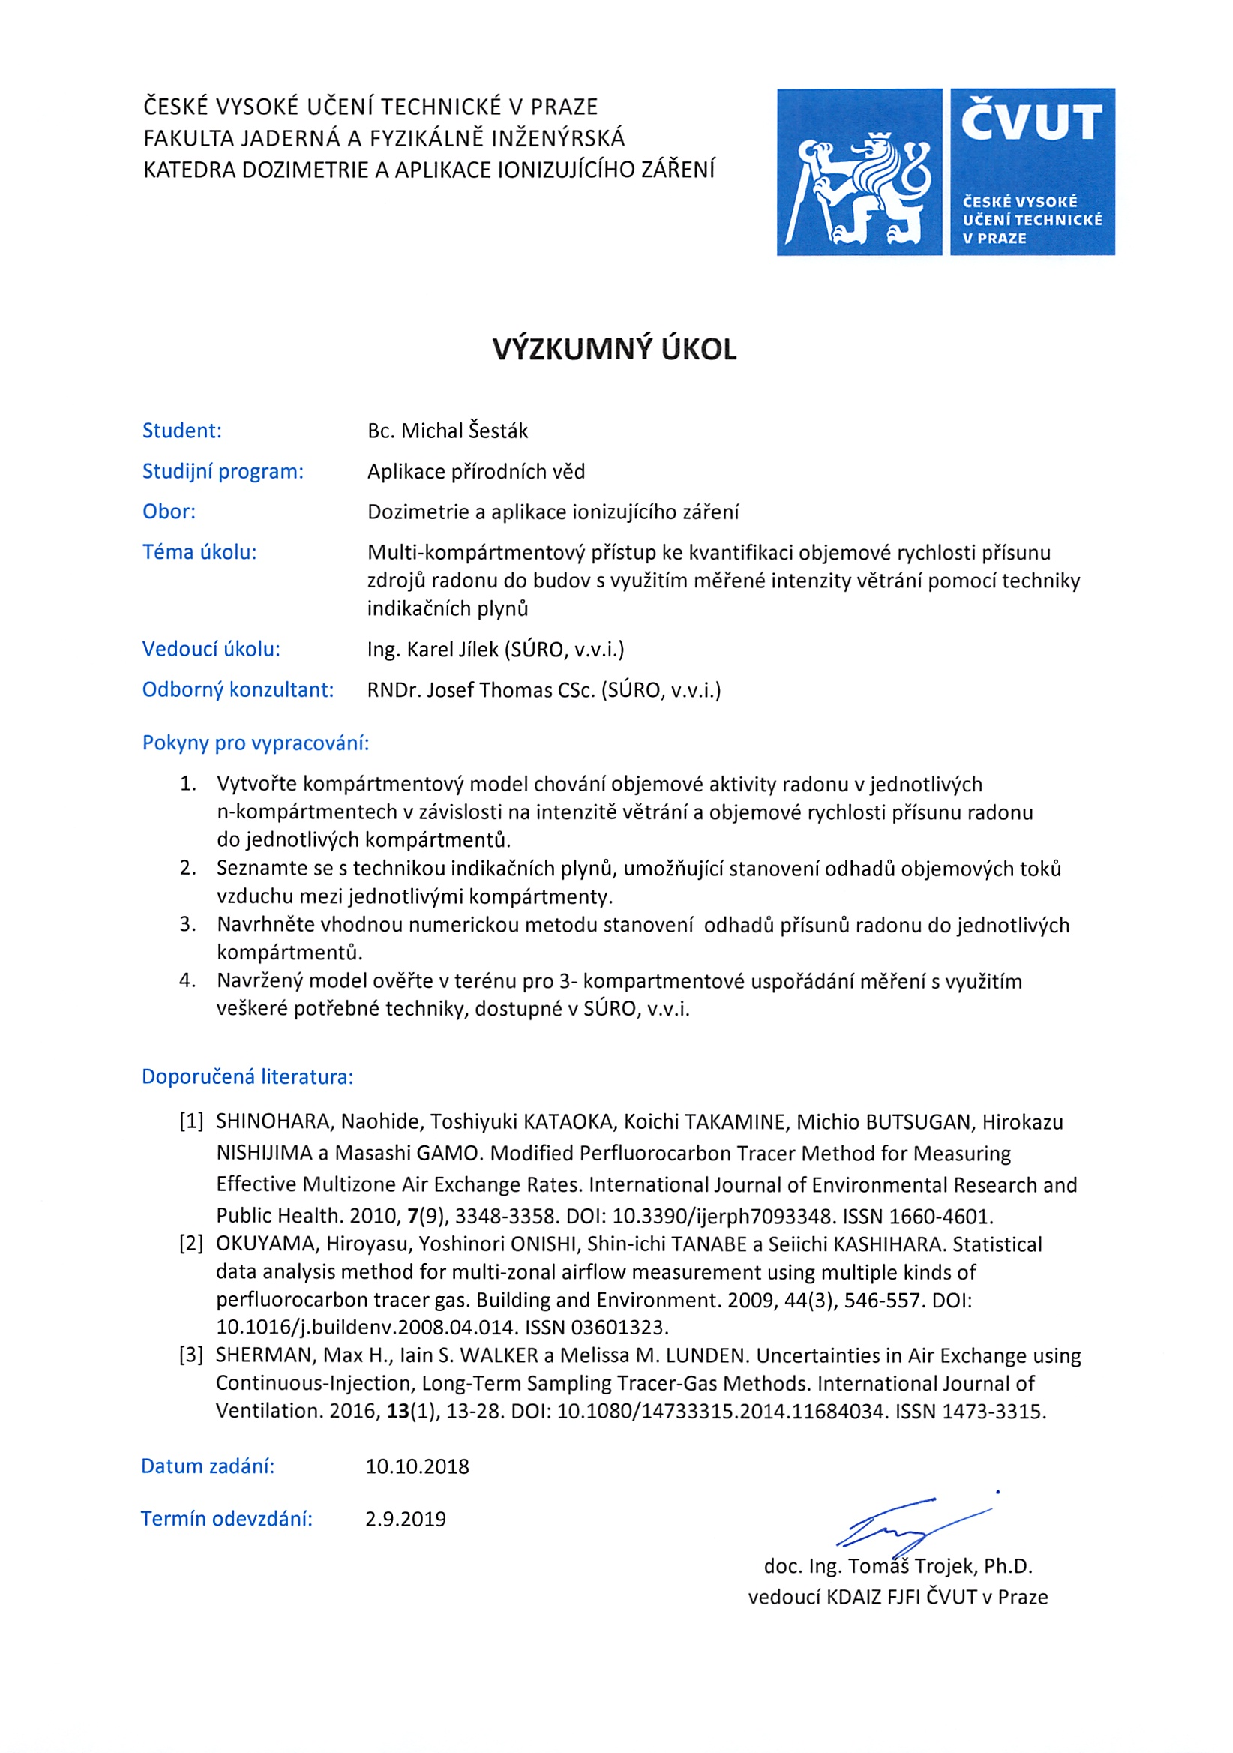
\includepdf[pages={1}]{zadani.pdf}
%\newpage
%\vspace*{\fill}
%\section*{Prohlášení}
%Prohlašuji, že jsem svůj výzkumný úkol vypracoval samostatně a použil jsem pouze podklady uvedené v přiloženém seznamu.\\[10pt]
%V Praze dne \\[10pt]
\newpage
\vspace*{\fill}
\section*{Poděkování}
Velmi děkuji panu Ing. Karlu Jílkovi za vedení mé práce. Také děkuji panu RNDr. Josefu Thomasovi, Csc. za přečtení a posouzení mé práce. Dále děkuji všem, kdo byli ochotni se se mnou o mém výzkumném úkolu bavit a odpovídat na mé dotazy. 
\newpage
\begin{tabularx}{\textwidth}{>{\itshape}l X}
  Název práce: & \textbf{Multi-kompártmentový přístup ke kvantifikaci  objemové rychlosti přísunu zdrojů radonu do budov s využitím měřené intenzity větrání pomocí techniky indikačních plynů}\\
  Autor: & Bc. Michal Šesták\\
  Obor: & Dozimetrie a aplikace ionizujícího záření\\
  Druh práce: & Výzkumný úkol\\
  Vedoucí práce: & Ing. Karel Jílek\\ 
               & Státní ústav radiační ochrana, v. v. i.\\
  Abstrakt: & <++>\\
  Klíčová slova: & radon, kontinuální měření radonu, měření ventilace, indikační plyny, objemové přísuny radonu, python  
\end{tabularx}
\newpage
\begin{tabularx}{\textwidth}{>{\itshape}l X}
  Title: & \textbf{<++>}\\
  Author: & Bc. Michal Šesták\\
  Abstract: & \\
  Key words: & 
\end{tabularx}
\newpage 
